% !TeX root = ../../thesis.tex
\chapter{Introduction}\label{ch:introduction}
%\chapter{Introduction}\label{ch:introduction}

This chapter aims to provide an overview of non-valence anions, with a specific emphasis on dipole-bound anions (DBAs). The relevance of these anions in biological systems is explored, followed by an introduction to the system of interest, namely biological quinones, and their critical role in biological processes. Finally, the research objectives are outlined.

\section{Non-Valence Anions}
An anion is an atom or molecule containing one or more excess electrons. Unlike valence electrons in neutral species, these "extra" electrons do not experience a -1/r Coulombic attraction at large distances and instead interact through weaker charge-multipole potentials.\cite{simons2008molecular, herbert2015quantum}.

In discussing molecular anions, the concept of electron affinity (EA) is fundamental. On one hand, the adiabatic electron affinity (AEA) quantifies the energy difference between the parent molecule and its corresponding anion, with both species in their electronic ground states and lowest rovibrational levels. On the other hand, the vertical electron affinity (VEA), is defined at the neutral equilibrium geometry, and is specially relevant for the dynamics of the electron capturing process. A molecule possessing a positive EA is considered electronically stable, as it necessitates an input of energy to remove an electron from the anionic state \cite{simons2008molecular}.

Molecular anions can be classified into two distinct categories: valence anions, where the excess electron occupies a compact orbital similar to the other valence molecular orbitals, and non-valence anions (NVA) \newglossaryentry{nva}{name={NVA},description={Non Valence Anion}}, where the excess electron occupies a diffuse orbital spatially separated from the molecule. These non-valence anions are further subdivided based on the predominant long-range interaction responsible for electron binding: dipole-bound states (DBS), quadrupole-bound states (QBS), and correlation-bound states (CBS).\cite{simons2008molecular,herbert2015quantum,abdoul1998electrons,simons2023molecular,jordan2003theory}.
The initial theoretical framework for non-valence bound states was proposed in 1947 by Fermi and Teller, who demonstrated that a dipole could bind an excess electron if the dipole moment surpasses 1.625 D \cite{fermi1947capture}. Further investigations refined the concept applying to "real" molecules, leading to a critical dipole moment of around 2.5 D\cite{jordan2003theory}.

Their ab initio descriptions often require particular attention due to the more diffuse nature of the associated orbitals \cite{simons2008molecular,simons2023molecular}. 
 Recent advances in spectroscopy have facilitated the study of NBS in the gas phase, generating significant interest in their properties \cite{kang2024reaction}. Additionally, solvated electrons, which may be considered a form of non-valence states, are hypothesized to reside in cavities approximately 2.5 \r{A} in size \cite{herbert2017hydrated}.

\subsection{Dipole-Bound Anions}
The theoretical investigation of DBAs presents two primary challenges. First, atomic orbital basis sets must be sufficiently diffuse to accurately describe the spatial extent of the DB orbital, often necessitating the use of custom basis sets \cite{skurski2000choose}. Although the electron in the DB orbital resides predominantly far from the precursor's valence electrons, it exhibits significant dispersion-like interactions with these electrons, contributing substantially to the electron binding energy (EBE). This interaction reflects the polarizable nature of the DB orbital, which engages in pronounced van der Waals interactions with nearby electron densities \cite{gutowski1996contribution}.

DBAs have garnered interest not only as theoretical constructs but also for their implications in diverse fields such as astrochemistry \cite{fortenberry2015interstellar} and radiation biology \cite{narayanan2023secondary,sedmidubska2024interaction}. Particularly intriguing are cases where the parent molecule also supports a valence anion state, allowing the DBA to act as a transition state for electron transfer to the more stable valence-bound anion (VBA).

When solvent effects are considered, distinct scenarios emerge. The electron may either (a) localize within the DB orbital, (b) be captured by solvent molecules forming a solvation cage, or (c) interact with solvent molecules whose instantaneous dipole orientations stabilize the DB state. The latter two phenomena are linked to charge-transfer-to-solvent (CTTS) electronic transitions \cite{bradforth2002excited,chen2000precursors}.

\subsection{Approaches to Study Non-Valence Anions}
Significant advancements have been achieved in experimental and theoretical methodologies for elucidating the structure and dynamics of NBS. Experimentally, high-resolution photodetachment and photoelectron spectroscopies, in conjunction with cryogenically cooled ion traps and velocity-map imaging, have enabled detailed characterization of NBS rovibrational structures. These techniques have proven instrumental in resolving sharp Feshbach resonances and identifying mode-specific vibrational autodetachment pathways.

The advent of time-resolved pump-probe photoelectron spectroscopy has further advanced the field by capturing ultrafast dynamics of electron detachment and transfer in NBS. Sub-picosecond timescales have been observed for electron transfer from DBS to valence-bound states in nucleobase-containing clusters, highlighting the transient role of NBS in electron-driven processes. Additionally, picosecond-resolved measurements have quantified autodetachment lifetimes in vibrationally specific manners, as demonstrated in phenoxide systems \cite{jordan2003theory,paran2024performance}.

Theoretical investigations have complemented experimental efforts through high-level quantum chemical techniques such as equation-of-motion coupled-cluster (EOM-CC) and density functional theory (DFT) \cite{thiam2023accurately}. Autodetachment processes have been modeled using Fermi's golden rule, with detachment rates linked to nuclear displacements of the electron-binding potential. These approaches have provided predictive frameworks for mode-specific detachment behaviors, particularly in DBS and QBS, where angular dependencies and induced dipole effects play critical roles.

\section{Non-Valence Anions in Biology}
Research on DBAs has predominantly focused on gas-phase systems. In biological contexts, DBAs have been studied for their interactions with DNA, particularly in radiation damage and radiosensitization \cite{narayanan2023secondary,sedmidubska2024interaction}. 

The survival of NBS in condensed matter remains a subject of debate. Computational studies suggest that hydration influences the localization of the excess electron, often displacing it onto the solvent cage's surface \cite{anusiewicz2020fate}. Conversely, experimental evidence indicates that alkyl chains do not disrupt DBS stability \cite{castellani2019stability}, and DBS-mediated mechanisms have been observed in solvated uracil systems \cite{narayanan2024electron}. The viability of NBS in bulk systems depends on the molecular density and polarity of the medium. While apolar solvents may hinder DBS existence due to excluded volume effects, polar solvents can stabilize DBS through dipolar interactions, analogous to CTTS states \cite{bradforth2002excited,chen2000precursors}.

The role of NBS in natural biological pathways remains largely unexplored. Their sensitivity to environmental factors suggests potential applications in regulating long-range electron transfer processes, particularly in soft matter systems such as proteins, which feature vacant pockets capable of accommodating DBS.

\subsection{Overlap with Biochemical Systems}
Studies on electron interactions with biomolecules, both in bare and hydrated states, have highlighted the significance of DBAs in biological systems \cite{gu2012interactions}. For instance, DBAs have been implicated in the electron transfer processes of flavins \cite{matthews2018observation}.

\section{Biological Quinones}
The term "quinone" originates from quinic acid, first identified in Cinchona bark in 1785 and later analyzed by Liebig \cite{chen2024low,rusell1873quinone}. Quinones are ubiquitous in biological systems and play vital roles as electron carriers in redox reactions \cite{ernster1995biochemical}.

\subsection{Role of Quinones}
Quinones facilitate electron and proton transfer between enzymes, serving as key intermediates in biochemical redox processes.

\subsection{Structural Aspects of Ubiquinone}
Coenzyme Q (ubiquinone), a prevalent quinone in nature, stabilizes both valence and dipole-bound anionic states due to its unique structure. This renders it an intriguing subject for NBS studies. Experimental observations have confirmed the presence of DBAs in 2-3-dimethoxy-para-benzoquinone (CoQ0), with diminished stability in CoQ1 and CoQ2 \cite{ameixa2023parent,west2014anion,pshenichnyuk2020ionizing,bull2015anion}.

% Some dummy code show how to include images.
\begin{figure}[th!]
  \centering
  \medskip
  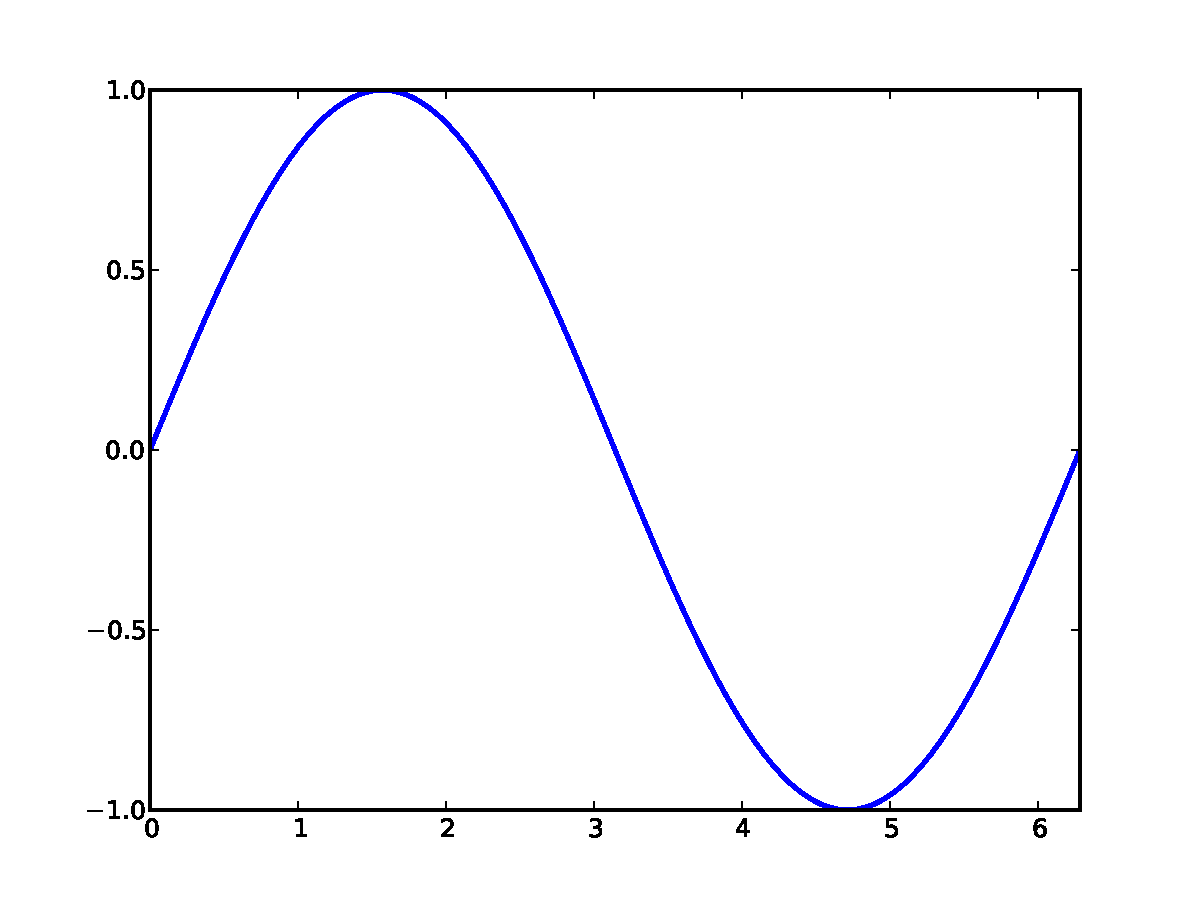
\includegraphics[width=.9\textwidth]{sine}
  \caption[Short caption for Table of Figures]{Illustration of how to
  include a figure (long text, should not go to Table of Figures).}
  \label{fig:sine}
\end{figure}

%Add list of symbols and abbreiations here:
% Some dummy code to get at least 1 entry in the nomenclature.
%\nomenclature{$\Theta$}{A nice symbol}
Introducing some symbol: $\Theta$.

% Some dummy code to get at least 1 entry in the list of
% abbreviations.
\newglossaryentry{md}{name={MD},description={molecular dynamics}}
Introducing an acronym: \gls{md}.

\begin{figure}[th!]
  \centering
  % GNUPLOT: LaTeX picture with Postscript
\begingroup
  \makeatletter
  \providecommand\color[2][]{%
    \GenericError{(gnuplot) \space\space\space\@spaces}{%
      Package color not loaded in conjunction with
      terminal option `colourtext'%
    }{See the gnuplot documentation for explanation.%
    }{Either use 'blacktext' in gnuplot or load the package
      color.sty in LaTeX.}%
    \renewcommand\color[2][]{}%
  }%
  \providecommand\includegraphics[2][]{%
    \GenericError{(gnuplot) \space\space\space\@spaces}{%
      Package graphicx or graphics not loaded%
    }{See the gnuplot documentation for explanation.%
    }{The gnuplot epslatex terminal needs graphicx.sty or graphics.sty.}%
    \renewcommand\includegraphics[2][]{}%
  }%
  \providecommand\rotatebox[2]{#2}%
  \@ifundefined{ifGPcolor}{%
    \newif\ifGPcolor
    \GPcolortrue
  }{}%
  \@ifundefined{ifGPblacktext}{%
    \newif\ifGPblacktext
    \GPblacktexttrue
  }{}%
  % define a \g@addto@macro without @ in the name:
  \let\gplgaddtomacro\g@addto@macro
  % define empty templates for all commands taking text:
  \gdef\gplbacktext{}%
  \gdef\gplfronttext{}%
  \makeatother
  \ifGPblacktext
    % no textcolor at all
    \def\colorrgb#1{}%
    \def\colorgray#1{}%
  \else
    % gray or color?
    \ifGPcolor
      \def\colorrgb#1{\color[rgb]{#1}}%
      \def\colorgray#1{\color[gray]{#1}}%
      \expandafter\def\csname LTw\endcsname{\color{white}}%
      \expandafter\def\csname LTb\endcsname{\color{black}}%
      \expandafter\def\csname LTa\endcsname{\color{black}}%
      \expandafter\def\csname LT0\endcsname{\color[rgb]{1,0,0}}%
      \expandafter\def\csname LT1\endcsname{\color[rgb]{0,1,0}}%
      \expandafter\def\csname LT2\endcsname{\color[rgb]{0,0,1}}%
      \expandafter\def\csname LT3\endcsname{\color[rgb]{1,0,1}}%
      \expandafter\def\csname LT4\endcsname{\color[rgb]{0,1,1}}%
      \expandafter\def\csname LT5\endcsname{\color[rgb]{1,1,0}}%
      \expandafter\def\csname LT6\endcsname{\color[rgb]{0,0,0}}%
      \expandafter\def\csname LT7\endcsname{\color[rgb]{1,0.3,0}}%
      \expandafter\def\csname LT8\endcsname{\color[rgb]{0.5,0.5,0.5}}%
    \else
      % gray
      \def\colorrgb#1{\color{black}}%
      \def\colorgray#1{\color[gray]{#1}}%
      \expandafter\def\csname LTw\endcsname{\color{white}}%
      \expandafter\def\csname LTb\endcsname{\color{black}}%
      \expandafter\def\csname LTa\endcsname{\color{black}}%
      \expandafter\def\csname LT0\endcsname{\color{black}}%
      \expandafter\def\csname LT1\endcsname{\color{black}}%
      \expandafter\def\csname LT2\endcsname{\color{black}}%
      \expandafter\def\csname LT3\endcsname{\color{black}}%
      \expandafter\def\csname LT4\endcsname{\color{black}}%
      \expandafter\def\csname LT5\endcsname{\color{black}}%
      \expandafter\def\csname LT6\endcsname{\color{black}}%
      \expandafter\def\csname LT7\endcsname{\color{black}}%
      \expandafter\def\csname LT8\endcsname{\color{black}}%
    \fi
  \fi
    \setlength{\unitlength}{0.0500bp}%
    \ifx\gptboxheight\undefined%
      \newlength{\gptboxheight}%
      \newlength{\gptboxwidth}%
      \newsavebox{\gptboxtext}%
    \fi%
    \setlength{\fboxrule}{0.5pt}%
    \setlength{\fboxsep}{1pt}%
    \definecolor{tbcol}{rgb}{1,1,1}%
\begin{picture}(4600.00,4320.00)%
    \gplgaddtomacro\gplbacktext{%
      \csname LTb\endcsname%%
      \put(714,562){\makebox(0,0)[r]{\strut{}$-1.5$}}%
      \csname LTb\endcsname%%
      \put(714,1156){\makebox(0,0)[r]{\strut{}$-1$}}%
      \csname LTb\endcsname%%
      \put(714,1749){\makebox(0,0)[r]{\strut{}$-0.5$}}%
      \csname LTb\endcsname%%
      \put(714,2343){\makebox(0,0)[r]{\strut{}$0$}}%
      \csname LTb\endcsname%%
      \put(714,2936){\makebox(0,0)[r]{\strut{}$0.5$}}%
      \csname LTb\endcsname%%
      \put(714,3530){\makebox(0,0)[r]{\strut{}$1$}}%
      \csname LTb\endcsname%%
      \put(714,4124){\makebox(0,0)[r]{\strut{}$1.5$}}%
      \csname LTb\endcsname%%
      \put(812,386){\makebox(0,0){\strut{}$-10$}}%
      \csname LTb\endcsname%%
      \put(1680,386){\makebox(0,0){\strut{}$-5$}}%
      \csname LTb\endcsname%%
      \put(2549,386){\makebox(0,0){\strut{}$0$}}%
      \csname LTb\endcsname%%
      \put(3417,386){\makebox(0,0){\strut{}$5$}}%
      \csname LTb\endcsname%%
      \put(4286,386){\makebox(0,0){\strut{}$10$}}%
    }%
    \gplgaddtomacro\gplfronttext{%
      \csname LTb\endcsname%%
      \put(3530,3965){\makebox(0,0)[r]{\strut{}$\sin(x)$}}%
      \csname LTb\endcsname%%
      \put(3530,3789){\makebox(0,0)[r]{\strut{}$\cos(x)$}}%
      \csname LTb\endcsname%%
      \put(3530,3613){\makebox(0,0)[r]{\strut{}$\tan(x)$}}%
      \csname LTb\endcsname%%
      \put(161,2343){\rotatebox{-270.00}{\makebox(0,0){\strut{}$y$}}}%
      \csname LTb\endcsname%%
      \put(2549,123){\makebox(0,0){\strut{}$x$}}%
    }%
    \gplbacktext
    \put(0,0){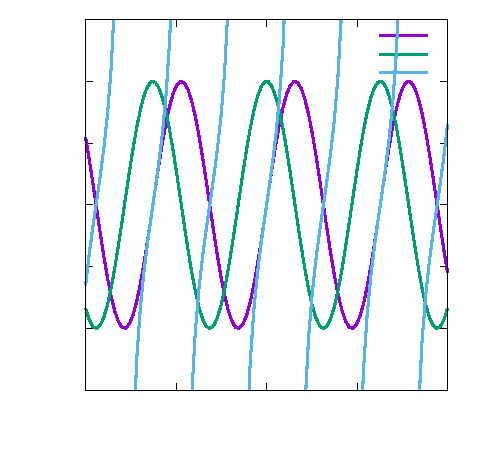
\includegraphics[width={230.00bp},height={216.00bp}]{test}}%
    \gplfronttext
  \end{picture}%
\endgroup

  %figsize is set in image/test.gp 
  \caption[Short caption for Table of Figures]{Illustration of how to
  include a figure (long text, should not go to Table of Figures).}
  \label{fig:test}
\end{figure}

%%%%%%%%%%%%%%%%%%%%%%%%%%%%%%%%%%%%%%%%%%%%%%%%%%
% Keep the following \cleardoublepage at the end of this file, 
% otherwise \includeonly includes empty pages.
\cleardoublepage

% vim: tw=70 nocindent expandtab foldmethod=marker foldmarker={{{}{,}{}}}
